\chapter{The Physics of OCE}\label{oce}

OCE can be thought of as the combination of a foundational imaging technique, optical coherence tomography, and its application to imaging mechanical properties: elastography. The underlying imaging technique, OCT, is discussed in \autoref{oct}, then OCE as a connected application of OCT and elastography in \autoref{application_elastography}. In \autoref{compression_oce}, the characteristics of a standard compression OCE system are discussed, as the one used in this project. As well, the implications of using phase-sensitive methods to measure displacement is discussed in \autoref{phase_sensitive}.

\section{Optical Coherence Tomography}\label{oct}
Optical coherence tomography (OCT) can be thought of as the optical equivalent to ultrasound, in that it detects the light reflected from scatterers within a tissue. The reflected light interferes with a reference beam, enabling depth-resolved reconstruction of the location of the scatterers within the sample \cite{chin_parametric_2016}. Because the speed of light in tissue is significantly higher than that of sound, OCT offers a much higher resolution than ultrasound, on the order of $5-15 \mu m$ \cite{kennedy_emergence_2017}, as limited by the coherence length of the light source \cite{huang_optical_1991}. However, this higher resolution comes at the expense of depth of penetration into the tissue, which for OCT, is only $1-2mm$ beneath the surface \cite{schmitt_optical_1999}, in comparison to the relatively deep imaging capabilities of ultrasound.

\begin{figure}
	\centering
    \begin{subfigure}{0.45\textwidth}
    	\centering
        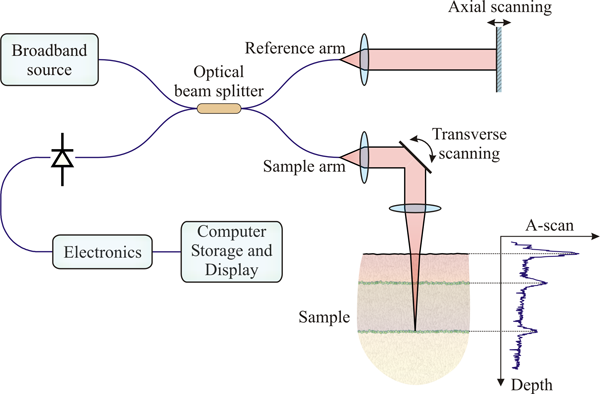
\includegraphics[width=\textwidth]{bground_figs/time_domain}
    \end{subfigure}
    \quad
    \begin{subfigure}{0.45\textwidth}
    	\centering
        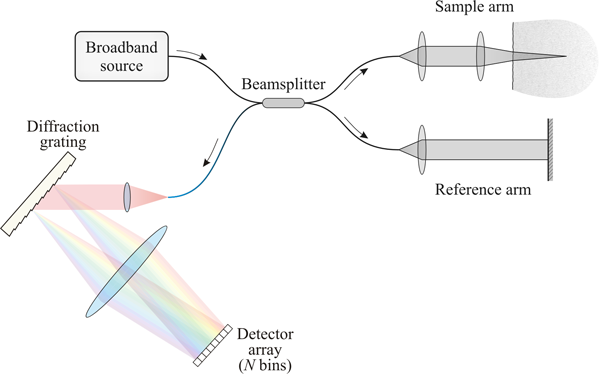
\includegraphics[width=\textwidth]{bground_figs/fourier_domain.png}
    \end{subfigure}
    \caption{Set ups for a) time-domain and b) Fourier-domain OCT systems. Taken from \cite{optical+biomedical_engineering_laboratory_introduction_nodate}.}
    \label{oct_domain}	
\end{figure}

\subsection{Time-Domain OCT}
Time-domain OCT uses a simple low coherence Michelson interferometer set up, as seen in \autoref{oct_domains}, where the interference signal is measured between the light reflecting from the tissue, and an scanned reference mirror that changes the depth imaged \cite{huang_optical_1991}. The scanning of the reference mirror to image into the tissue produces a 1D A-scan, that contains information about the detected irradiance of the interferometer as a function of depth. Taking multiple A-scans across by moving laterally across a sample surface produces a 2D B-scan. Multiple B-scans can be used as cross-sections to build up an entire 3D scan volume, otherwise known as a C-scan, a process which can be seen in Figure 2. These descriptions are taken from those conventionally utilised in ultrasound imaging. The disadvantage of this set up however is the expensive acquisition times for imaging of 3D volumes.

\subsection{Fourier-Domain OCT}
Fourier-domain OCT systems remove the need for a scanning mirror, and allows the reproduction of a single A-scan with one detection event based on principles of spectral interferometry \cite{chin_parametric_2016}. Rather than detecting the reflected intensity as a function of depth as in time-domain OCT, it is detected as a function of wavenumber of a broadband or swept frequency light source. The Wiener-Khinchin theorem dictates that the inverse Fourier transform of this measured spectral density provides the complex coherence function at different depths along the A-scan line \cite{schmitt_optical_1999}. The speed up using Fourier-domain OCT over time-domain OCT allows the imaging of 3D volumes, of approximately $10mm \times 10mm \times 2mm$ to be acquired in less than 1 second \cite{kennedy_emergence_2017}. The benefit of Fourier-domain OCT over time-domain is not only in allowing a much faster acquisition time, but it also produces a complex signal that carries phase information, allowing it to be used as to quantify displacement within a sample, as described in \autoref{phase_sensitive}.

\subsection{Speckle in OCT}
\begin{itemize}
	\item Coherent imaging technique (constructive interference of a broadband light source)
	\item NOTE - where broadband source removes periodicity of constructive/destructive interference pattern
	\item Detects reflection from scatterers within a tissue (i.e. net scattering vector produced by difference in refractive indices - otherwise scatterers are randomly oriented within a volume of uniform optical properties/refractive index)
	\item Coherence length (range within which matches and produces an intensity maximum) is defined by the size of the frequency bandwidth of the laser used. This defines the optical resolution of the system.
	\item COHERENCE LENGTH IN OUR SYSTEM?
	\item Since this intensity pattern is dependent on the intensity of the constructive interference with reference and backscattered light field, a higher intensity implies a better match, and suggests that the estimate of displacement in that region (determined by assessing the 'position' of the reference arm) more accurately specifies the location of the scatterers within the volume.
	\item Think of this as a random phasor?? Where the intensity = addition of both, has associated phase, but added to this is random phasor sum of sub-resolution scatterers (see paper about this).
\end{itemize}

\section{Application to Elastography}\label{application_elastography}

Many elastography methods based on optical imaging techniques exist, and can be differentiated between by examining how the mechanical load is applied to the tissue, as well as what parameter is utilised to form the image, or 'elastogram' (as discussed in \autoref{elastography}). These different factors, as well as the underlying imaging technique, determine the resolution and penetration of the resulting imaging. In addition these parameters may be quantitative or qualitative, which has implications for diagnostic capability, and mechanical loading methods can be simple or complex, which introduces limitations on image acquisition time.

\begin{figure}[t]
	\centering
    	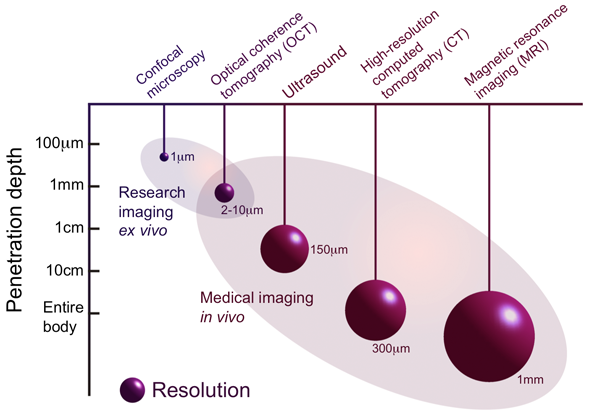
\includegraphics[width=0.7\textwidth]{bground_figs/technique_comparison.png}
    	\caption{Relative resolutions and penetrations for different imaging techniques utilised clinically, taken from \cite{optical+biomedical_engineering_laboratory_introduction_nodate}}
    	\label{image_techniques}	
\end{figure}

On top of these highly variable loading methods, the detection of tissue deformation can be done using speckle tracking via cross-correlation algorithms (which are highly influenced by speckle decorrelation noise), or by phase-sensitive detection \cite{kennedy_strain_2012}.

Optical coherence elastography (OCE) is the combination of elastography with an OCT imaging system, as first proposed by Schmitt in 1998 \cite{schmitt_oct_1998}. The micro-architecture of tissue carries important information about disease states, however these are poorly demonstrated using only optical contrast. Using elastography with optical coherence tomography as the underlying imaging modality allows high mechanical contrast imaging on scales previously inaccessible to ultrasound and MRI-based elastography techniques (see \autoref{image_techniques}). Of particular interest in this project is compressive OCE utilising phase-sensitive detection. 

\section{Compression OCE}\label{compression_oce}    

% Describe compression OCE in more detail ->
Compression OCE systems introduce a mechanical load to the sample by applying force to it in the axial direction, which results in displacement of the tissue, dependent on its constituent elastic properties. The typical system set up can be seen in \autoref{oce_system}.

Compression OCE produces a displacement field in the tissue, that can be measured in order to calculate the strain present. The local strain is estimated as the spatial derivative of these displacements with respect to depth \cite{kennedy_review_2014} over a given axial fit window. For phase-sensitive compression OCE, this displacement is directly related to the phase difference between an unloaded (not compressed) and loaded (compressed) scan, by Equation 2 \cite{kennedy_strain_2012}. However compressive loading techniques provide only qualitative comparison in strain elastograms, since it is dependent on the amount of compressive loading applied to the tissue. It is possible to produce quantitative elastogram images by measuring the stress locally applied to the sample by introducing a known stress layer above the imaged sample, as discussed in detail in \cite{kennedy_quantitative_2015}, however this will not be discussed further here. The benefit of compression techniques is their fast acquisition speeds for entire 3D volumes, as well as their ability to be extended to needle based OCE systems for imaging deep within the tissue \cite{kennedy_review_2014}. 

\begin{figure}
	\centering
	\begin{subfigure}{0.4\textwidth}
    	\centering
        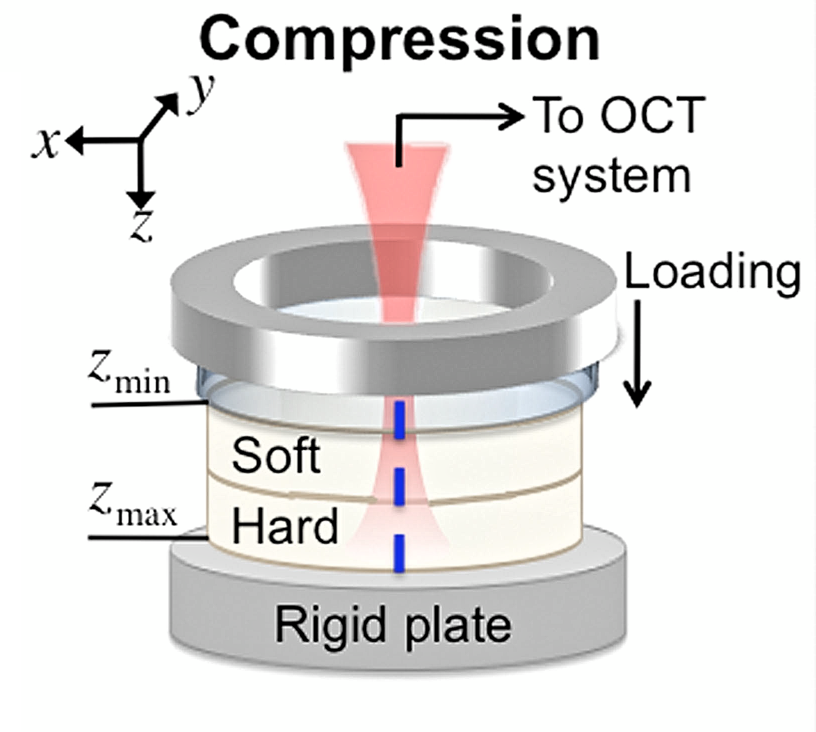
\includegraphics[width=\textwidth]{bground_figs/oce_hardware.png}
    \end{subfigure}
    \begin{subfigure}{0.3\textwidth}
    	\centering
        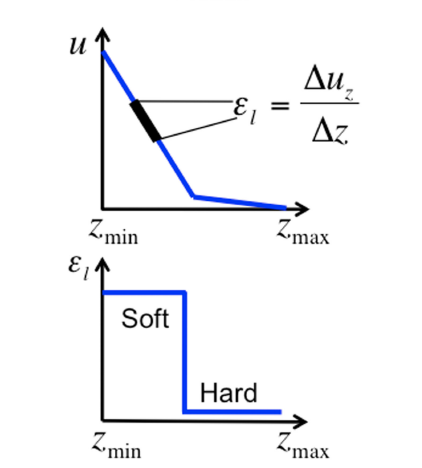
\includegraphics[width=\textwidth]{bground_figs/ascan_example.png}
    \end{subfigure}
    \label{oce_system}
\end{figure}

The OCT system produces a complex data value for each voxel inside the imaged volume, which has an amplitude associated with the optical intensity of the backscattered light at that point. The signal also has an associated phase, which is random. Altough the phase is random at each point in space, the change in phase is directly proportional to the amount the tissue is displaced at that location. Therefore there is a direct relationship between the displacement field and these measured phase differences.
The OCT signal can be thought of as a constant vector, representing the true signal due to a single reflection from the tissue at the given depth, with an attached random phasor sum, representing multiple scattering events within the tissue that introduce noise \cite{goodman_statistical_2015}. To reduce the influence of this approximately Gaussian noise attached to the signal, the complex signal is averaged over multiple B-scans before processing. Therefore each loaded and unloaded phase value actually corresponds to a chunk of values taken at multiple points across the y-axis. 

\begin{equation}
u_i = \frac{\phi_i^{loaded}-\phi_i^{unloaded}}{4\pi n} = \frac{\Delta\phi_i}{4\pi n}
\end{equation}

OCE inherits the high spatial resolution of the underlying OCT imaging system, however the strain estimation process that is applied to the phase-sensitive data has the potential to degrade this slightly, although still allowing imaging of tissue micro-architecture. However OCE also maintains the low penetration depth of OCT imaging, making the need for intra-operative OCE set ups, capable of scanning deep tissue temporarily exposed in surgery, even more essential. 

\section{Phase-Sensitive Displacement Measurement}\label{phase_sensitive}

\begin{figure}[t]
	\centering
	\begin{subfigure}{0.49\textwidth}
		\centering
		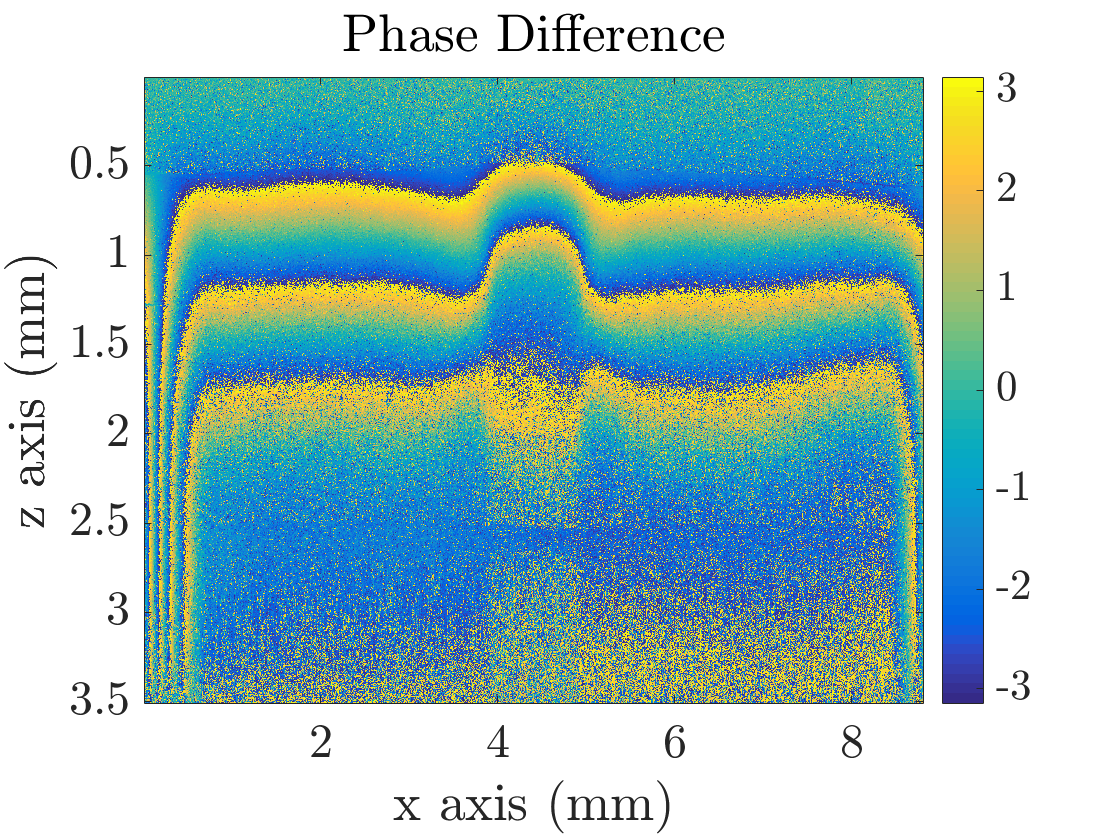
\includegraphics[width=\textwidth]{bground_figs/phase_difference.png}
	\end{subfigure}
	\begin{subfigure}{0.49\textwidth}
		\centering
		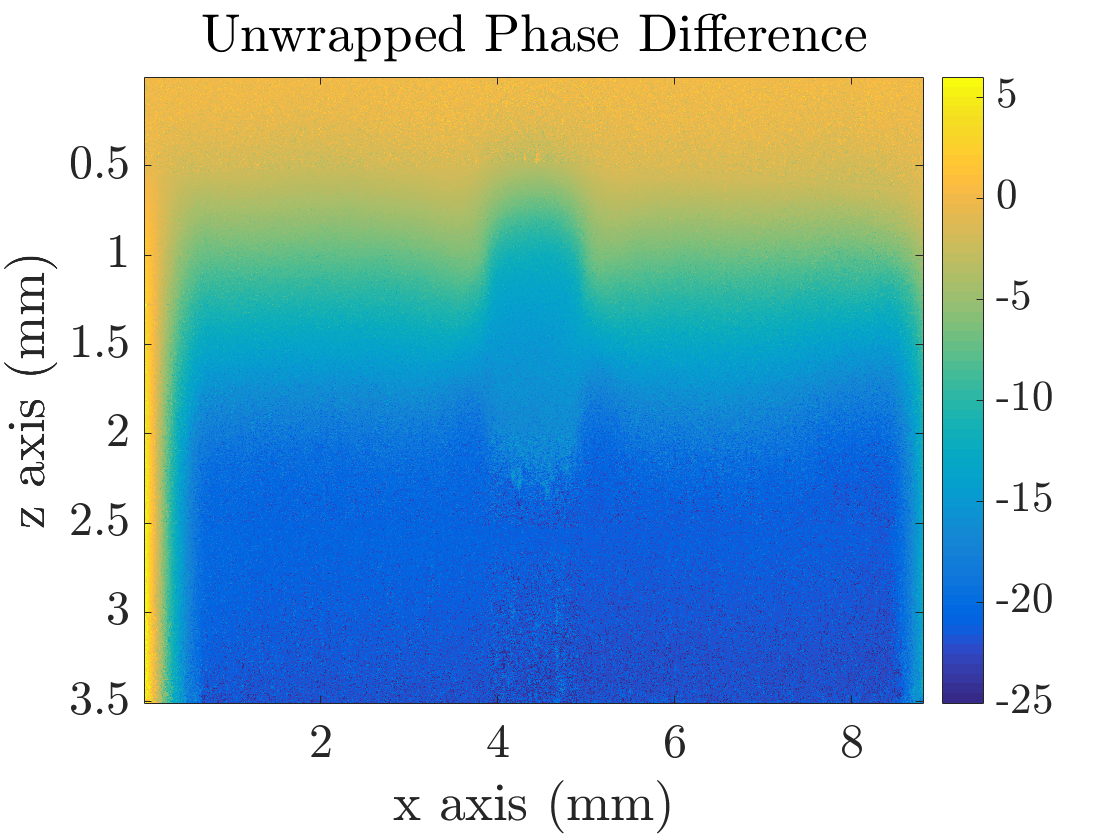
\includegraphics[width=\textwidth]{bground_figs/unwrapped_phase.png}
	\end{subfigure}
	\caption{Phase unwrapping demonstrated in a phantom scan data set in a) followed by the unwrapped phase difference b) computed using the unwrapping algorithm from \cite{kennedy_optical_2014}.}
	\label{phase_wrapping}	
\end{figure}

The efficiency of any elastography imaging technique is dependent on its ability to measure the deformation of the tissue in response to the mechanical load accurately. Phase-sensitive displacement measurement in OCE is enabled by Fourier-domain OCT systems, and allows tissue displacements on the order of nanometres to be detected by the system, corresponding to micro-strain sensitivity \cite{kennedy_review_2014}. However phase-sensitive OCE methods bring with them their own problems, one being that te detected phase can only take values in the interval $[0,2\pi]$. This results in wrapping of the phase difference as seen in \autoref{phase_wrapping} and if uncorrected, will result in discontinuities in the calculated displacement field.

\subsection{Phase Unwrapping}
To prevent phase wrapping in phase-sensitive displacement measurements, the difference in displacement between loaded and unloaded scans must be limited to approximately $0.3-0.46\mu m$ \cite{kennedy_optical_2014}. However in most instances, the amount of compression applied in OCE in order to produce images with sufficient contrast results in displacements large enough to induce phase wrapping in the signal. Therefore the issue of phase wrapping must be tackled in some way. Three different techniques of phase unwrapping are discussed in this project. The first technique is to implement a phase unwrapping algorithm that loops through the data set and detects wrapping events. This algorithm is more completely described in the paper \cite{kennedy_optical_2014} (see section 2.5) however at a high level, it works under the assumption that displacements induced at a given depth is uniform over a local region, and performs first axial then lateral unwrapping. The phase difference is assumed to be unwrapped over an initial depth segment, for which a mean phase value is calculated. From here, each subsequent voxel in depth has an integer number of $2\pi$ subtracted from it based on minimising the difference between its phase value and the preceding mean value, in order to axially unwrap. The lateral unwrapping is performed in a similar way, except by minimizing the difference between the phase at a given voxel with the averaged phase of its lateral neighbours. It has been demonstrated that the algorithm can remove up to 5 wrapping discontinuities \cite{kennedy_optical_2014} before artefacts become prominent.
The benefit of the phase unwrapping algorithm is that it is capable of returning the reconstructed displacement field of the entire B-scan. 

\begin{figure}[b]
	\centering
	\begin{subfigure}{0.25\textwidth}
		\centering
		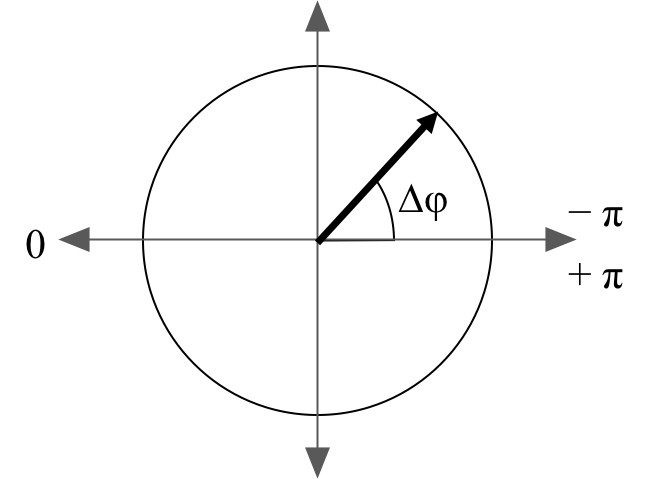
\includegraphics[width=\textwidth]{bground_figs/cplx_phasedif_phasor.png}
	\end{subfigure}
	\quad
	\begin{subfigure}{0.25\textwidth}
		\centering
		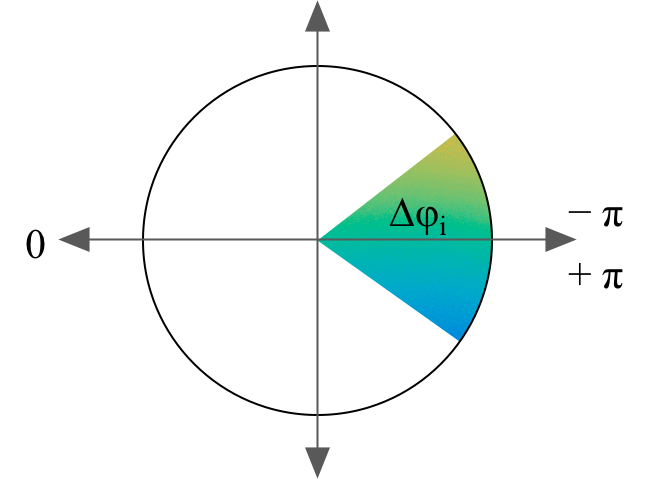
\includegraphics[width=\textwidth]{bground_figs/cplx_phasedif_segment.png}
	\end{subfigure}
	\quad
	\begin{subfigure}{0.25\textwidth}
		\centering
		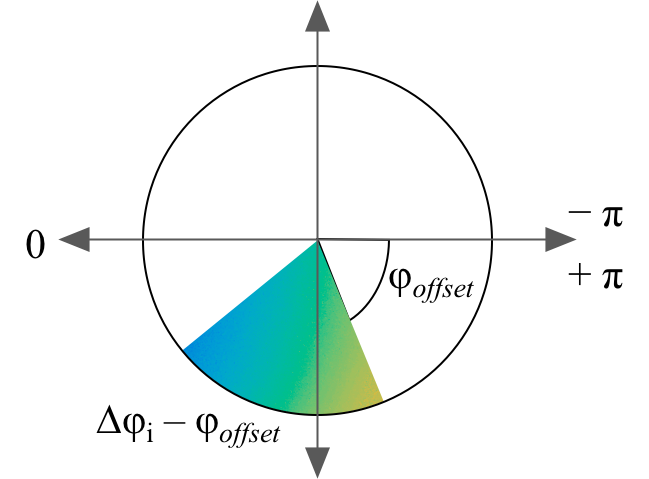
\includegraphics[width=\textwidth]{bground_figs/cplx_segment_shifted.png}
	\end{subfigure}
	\caption{The complex phase difference signal using phasor representation in a) as a single data point, b) as a fit window of phase difference data points wrapped around the $\pi/\pi$ discontinuity, and c) those data points shifted to an unwrapped region, based on application of a phase offset \cite{zaitsev_hybrid_2016}.}
	\label{phase_offset}	
\end{figure}

\subsection{Phase Offset Correction}
An alternative approach to the phase wrapping issue was investigated by Zaitsev et.al. \cite{zaitsev_hybrid_2016}, based on the fact that the underlying displacement field does not have to be extracted for the entire scan to produce a strain elastogram, but alternatively only the gradient within the fitting window must be maintained and extracted. In this case the phase unwrapping algorithm is dropped, and a complex phase offset is subtracted from each fit segment to remove any possible wrapping event by returning it to an unwrapped region, as shown in \autoref{phase_offset}. From here the strain is estimated using the unwrapped fit segment. This method obviously falters when there are multiple wrapping discontinuities within a given strain fit window, however this is unlikely given most strain estimation techniques maintain smaller fit windows to increase the resulting axial resolution.
Subtraction of a complex phase offset is a non-linear filter operation, and therefore must be performed on each fit segment separately. For strain estimation filter methods (discussed in \autoref{review}) this bottleneck slows down the strain estimation process for methods that use a phase offset to unwrap, however it can be mitigated by methods described in the next section.

\subsection{Alternative Approaches}
A third range of approaches do not tackle the issue of phase unwrapping directly, but rather makes the fit segment so small it is assumed no wrapping can occur between. Using finite difference to calculate the strain, performed on the complex phase, ensures that no wrapping artefacts enter the image, provided that no wrapping events occur between consecutive pixels, which is a valid assumption with the amount of compression used. The down side to this technique is that finite difference and any other technique that uses a very small fit window to mitigate phase unwrapping issues is a noisy differentiation method, and results in significant degradation of image quality when used alone. The following Chapter discusses such strain estimation methods in more detail, separate to the issue of phase unwrapping.


